\documentclass{beamer}
\usetheme{default}
\useoutertheme{miniframes}
\useinnertheme{circles}

\usepackage{hyperref}
\usepackage{pgf}  
\logo{\pgfputat{\pgfxy(-11, 0)}{\pgfbox[center,base]{
\includegraphics[width=2.5cm]{ANUlogo.png}}}} 

\definecolor{ANUbg}{rgb}{0.2, 0.2, 0.2}
\definecolor{ANUblue}{rgb}{0.56, 0.69, 0.75}
\usecolortheme[named=ANUbg]{structure}

\title{Machine Learning Approaches to Computational Protein Design}


\author{Stephen Zhang}

% Let's get started
\begin{document}

\begin{frame}
  \titlepage
\end{frame}

\section{Introduction}

\begin{frame}
    \begin{itemize}
        \item Computational techniques can be used to design mutant aaRS that exhibit affinity and specificity for corresponding uAAs.
        \item Major utility of computational protein design - \textit{huge reduction of search space}
        \item \texttt{Rosetta} is a state-of-the-art software package for a wide range of protein computation protocols.
    \end{itemize}
\end{frame}

\begin{frame}
    Conventional workflow is as follows...
    \begin{enumerate}
        \item Construct protein model (e.g. \textit{Mj}TyrRS, pCNFRS) based off crystal structures. Place uAA in binding site, specify mutation sites and kinetic constraints.
        \item Generate mutant candidates using \texttt{Rosetta} protocols. Calculate various score factors for mutants.
        \begin{center}Mutant pose $\to$ $\mathrm{scores}(E_1, E_2, E_3, ...)$\end{center}
        \item Select candidates for \textit{in vitro} experimentation by applying thresholds or ranking w.r.t several score factors, e.g. $\underbrace{\text{total score} > E_0}_{\text{a rectangular constraint!}}$
    \end{enumerate}
\end{frame}

\begin{frame}
    This has significant limitations: boundary between 'good' and 'bad' may be nonlinear! \\
    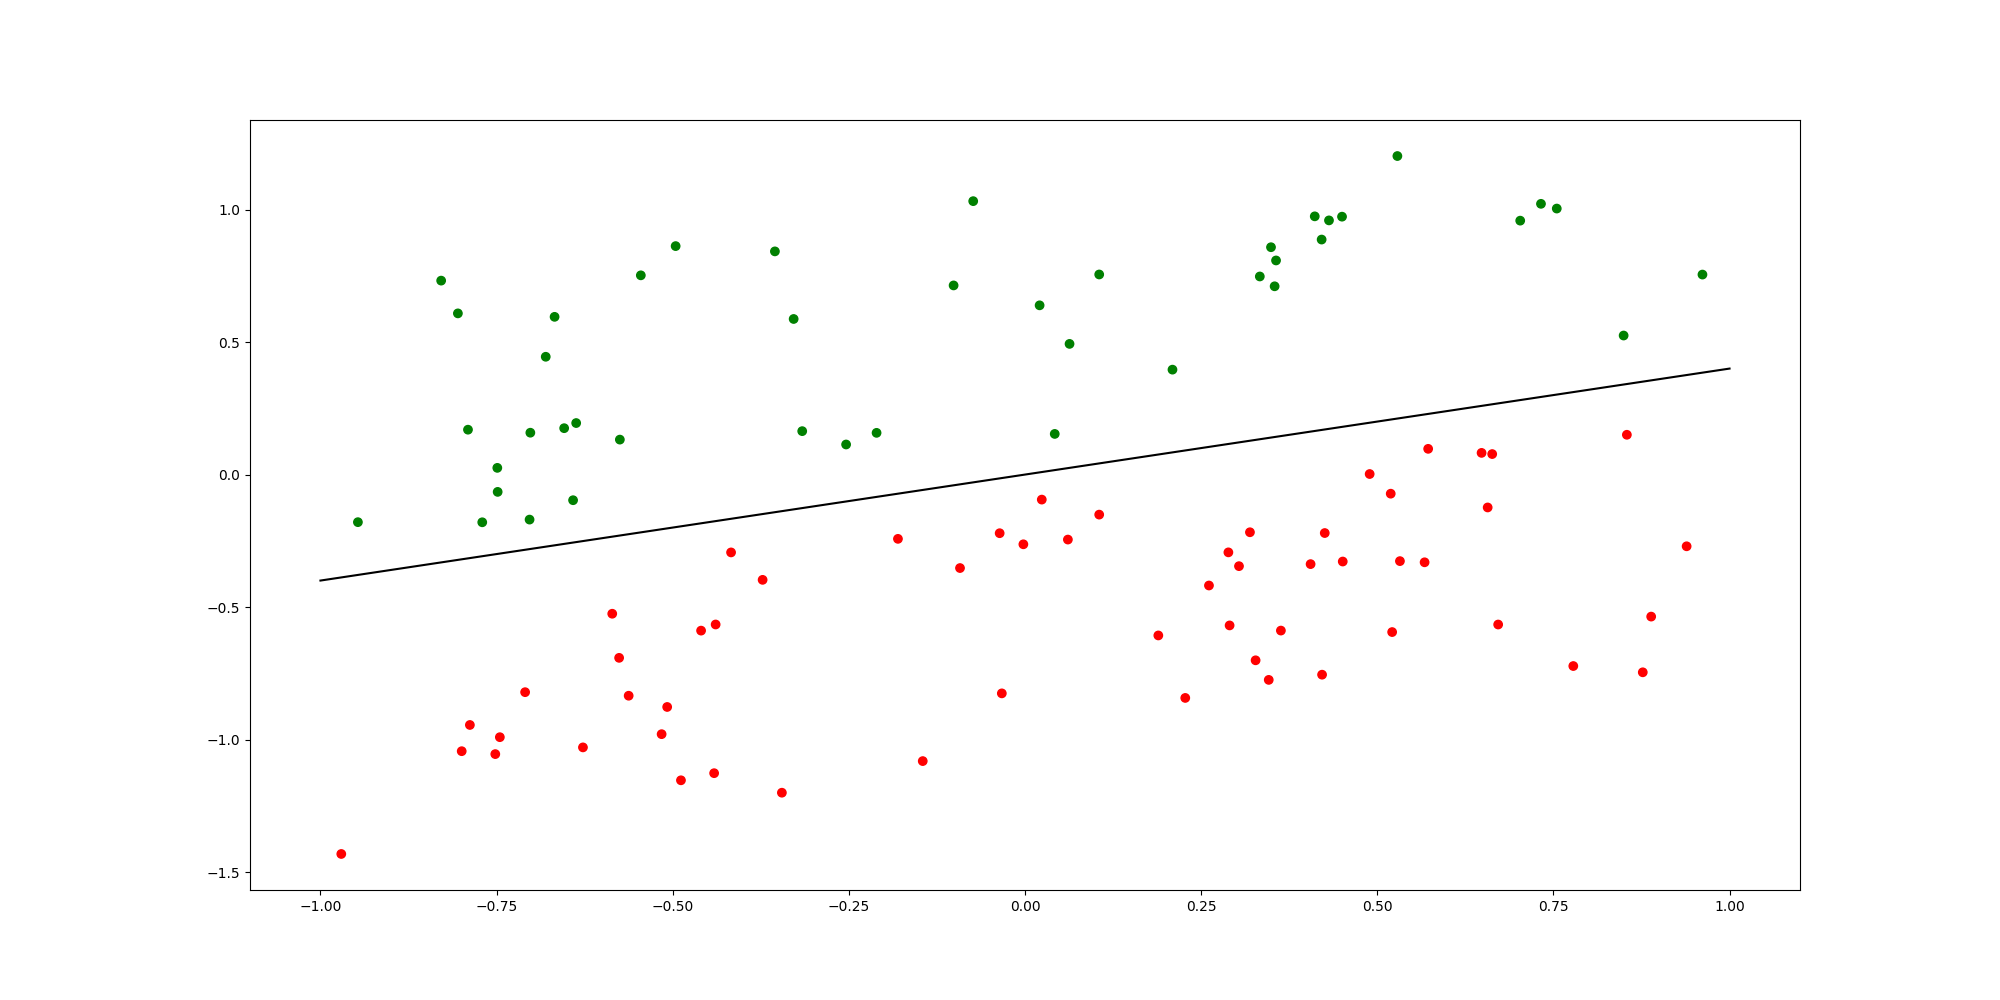
\includegraphics[width=\linewidth]{diagram1.png}
\end{frame}
\begin{frame}
    This has significant limitations: boundary between 'good' and 'bad' may be nonlinear! \\
    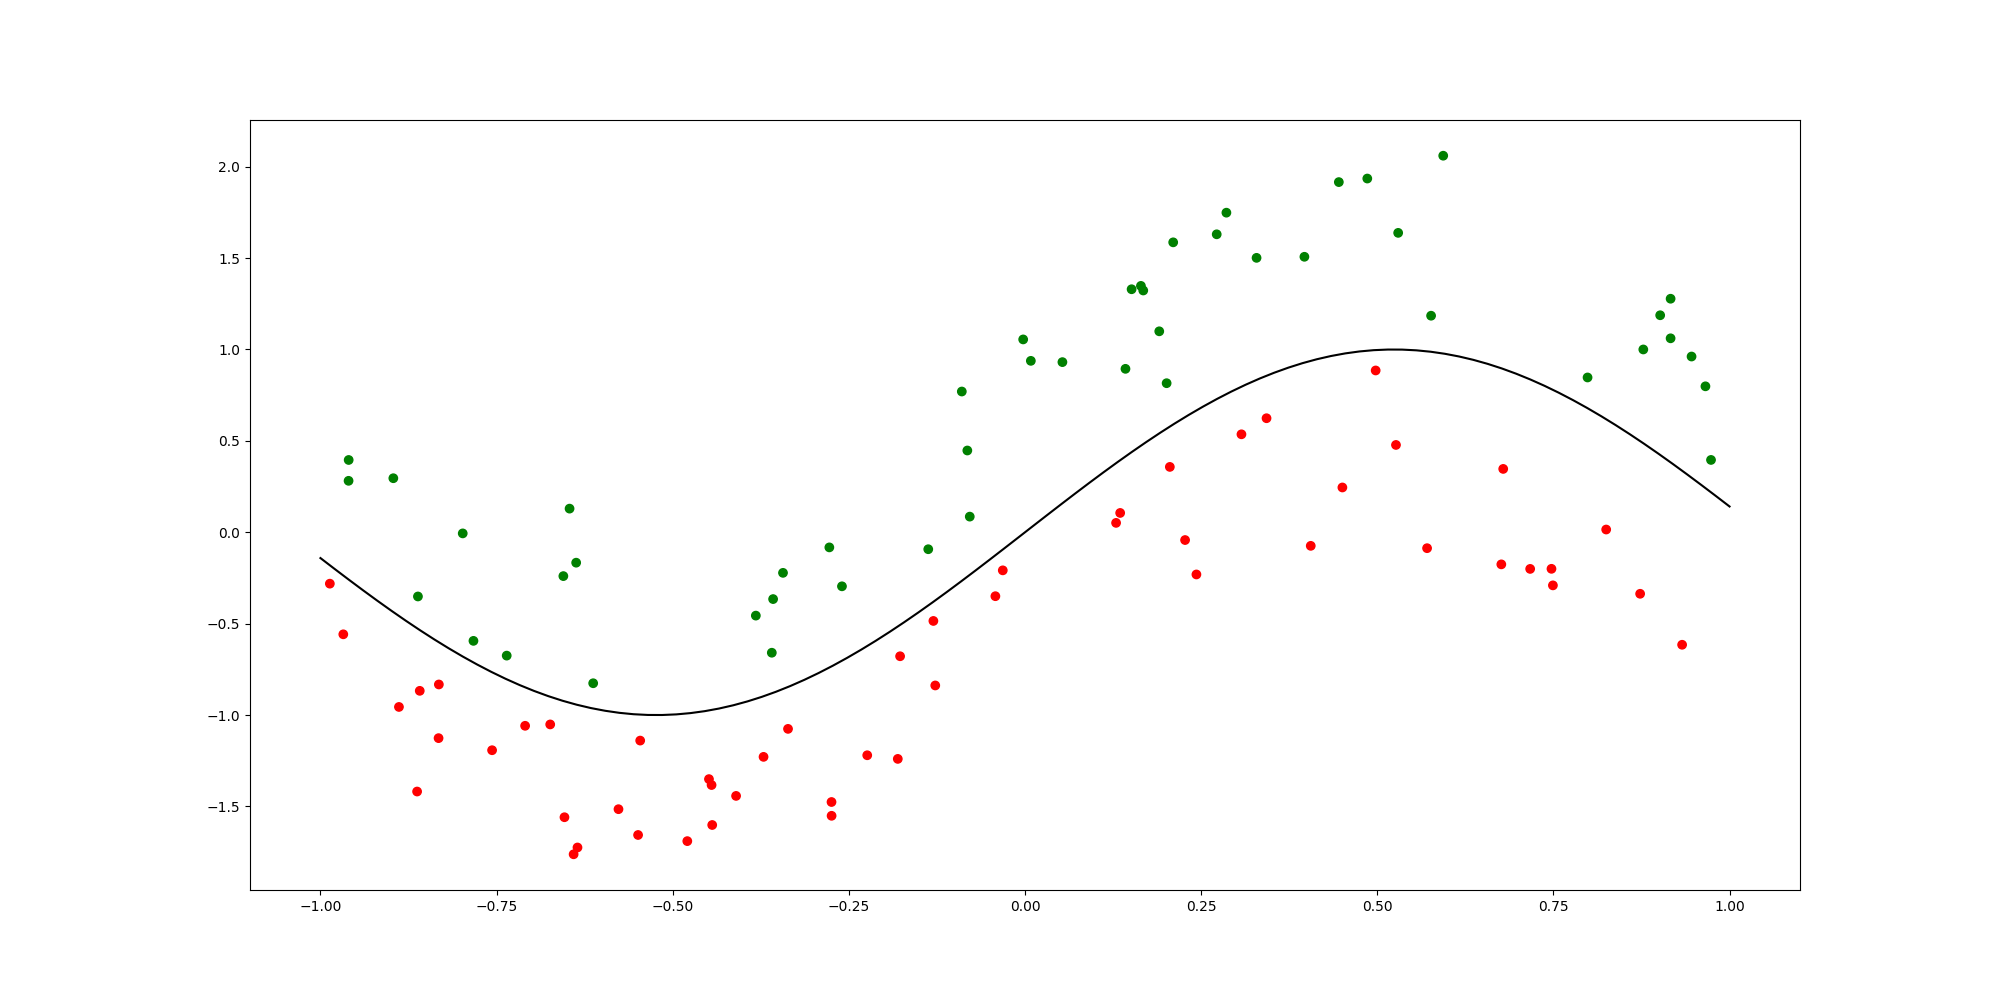
\includegraphics[width=\linewidth]{diagram2.png}
\end{frame}

\begin{frame}
    Machine learning techniques, specifically \textbf{binary classifiers}, can be used to deal with these situations.
\begin{enumerate}
\item For each candidate protein, we have a set of \texttt{Rosetta} scores \texttt{fa\_atr}, \texttt{fa\_sol}, ...
    These are called \textbf{factors}. Any candidate mutant is described by a vector of factors in a high-dimensional space:
    $$\vec{x} = (E_1, E_2, E_3, ..., E_m)$$
    
    \item Each candidate mutant is associated with its \textbf{class} $\in \{0, 1\}$. Here, 0 = 'non binding', 1 = 'binding'. We seek a map $F : \vec{x} \in \mathbb{R}^m \to \{0, 1\}$ that can predict \textbf{class} from \textbf{factors}.
    
    \item Machine learning methods allow approximations for such a function $F$ to be iteratively \textbf{learned} by a computer.
\end{enumerate}
\end{frame}

\begin{frame}
    Three binary classification approaches were employed, implemented in Python using \texttt{sklearn} library.
    \begin{enumerate}
        \item Logistic regression | linear model
    \item Artificial neural network (ANN) | nonlinear model
        \item Support vector machine (SVM) | nonlinear model
    \end{enumerate}
\end{frame}

\section{Methods}
\begin{frame}{Training set}
    Training set comprised of uAA's reported in literature be incorporated by \textit{Mj}TyrRS or \textit{p}CNFRS.
    \begin{itemize}
        \item Dumas et al., \textit{Chem. Sci.}, 2015, 6, 50 $\rightarrow$ 60 mutant-uAA pairs
        \item From previous work in Huber group...
        \item Nitroxide-incorporating \textit{p}CNFRS mutants $\rightarrow$ 28 mutants
        \item O-tert-butyl tyrosine incorporating \textit{p}CNFRS mutants $\rightarrow$ 14 mutants
    \end{itemize}
\end{frame}

\begin{frame}{Protocol}
    For consistency, all mutants were modelled on \textit{p}CNFRS (PDBID \texttt{3QE4}).
    \begin{itemize}
        \item For all mutants, 200 conformers of uAA and TYR generated using \texttt{balloon}, \texttt{Rosetta} \texttt{.params} file generated using \texttt{molfile\_to\_params.py}
        \item uAA and TYR positioned in binding pocket using \texttt{pymol}
        \item Mutated residues were specified, inputs passed to \texttt{EnzymeDesign} application. 500 decoys generated \textit{each} for mutant-uAA and mutant-TYR $\rightarrow$ score data!
\end{itemize}
\end{frame}

\begin{frame}{Input dataset is chemically diverse}
\begin{center}
    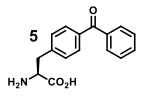
\includegraphics[scale = 0.5]{uAA1.png}
    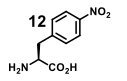
\includegraphics[scale = 0.5]{uAA2.png}
    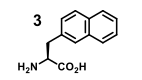
\includegraphics[scale = 0.5]{uAA3.png}
    \\
    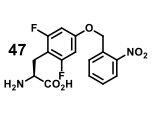
\includegraphics[scale = 0.5]{uAA4.png}
    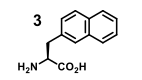
\includegraphics[scale = 0.5]{uAA5.png}
    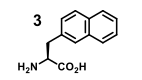
\includegraphics[scale = 0.5]{uAA6.png}
\end{center}
\end{frame}

\begin{frame}{Training and testing}
    
\end{frame}
\end{document}


